\documentclass{article}
\usepackage{amsmath}
\usepackage{hyperref}
\usepackage{graphicx}

\begin{document}
\paragraph{}
Hello dear Planeswalker, look at this graph for it may catch your interest.

\paragraph{}
\url{https://www.desmos.com/calculator/1o7625bms4}

\paragraph{}
Function $f(x,q,w,n,N)$ shows probability of getting specific number of cards
when pulling from deck of MTG cards.

\paragraph{}
Where:
\begin{description}
    \item[$x$] -- broj karata od interesa,
    \item[$q$] -- minimalni broj karata koji želimo povući (od x mogućih),
                  $q\leq n$,
    \item[$w$] -- maksimalni broj karata koji želimo povući, $q\leq w\leq n$,
    \item[$n$] -- broj karata koje se izvlače (npr. za prvi red $7$ ili $8$),
                  $n > 0$,
    \item[$N$] -- broj karata u deku (npr. $60$), $N > 0$.
\end{description}




$$
f(x, q, w, n, N) = 
\sum_{\substack{q\leq j\leq w}}
\left(
\frac{n!}{j! (n-j)!} \cdot
\prod_{\substack{0\leq i< n}}
\frac{1}{N-i} \cdot
\prod_{\substack{0\leq i< j}}
(x-i) \cdot
\prod_{\substack{0\leq i< n-j}}
(N-x-i)
\right)
$$

written without products:

$$
f(x, q, w, n, N) = 
\sum_{\substack{q\leq j\leq w}}
\left(
\frac{n!}{j! (n-j)!} \cdot
\frac{(N-n)!}{N!} \cdot
\frac{x!}{(x-j)!} \cdot
\frac{(N-x)!}{(N-x-n+j)!}
\right)
$$

$f(x, 3, 7, 7, 60)$

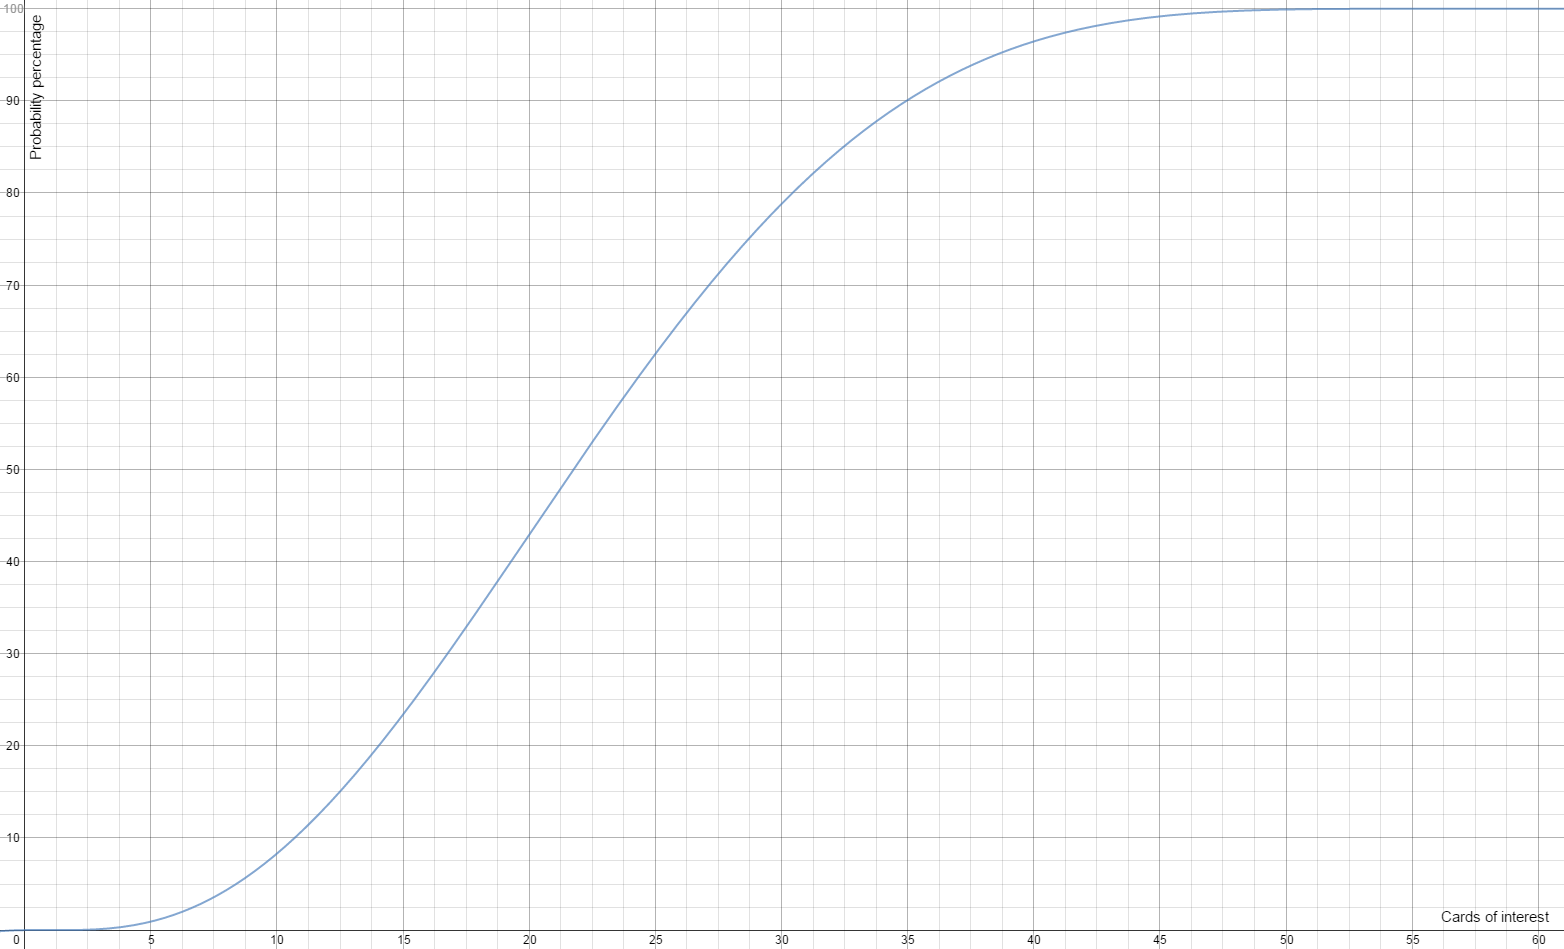
\includegraphics[width=\linewidth]{img/x_03_07_07_60_20141125_01.png}

\end{document}